\section*{Appendix}

\subsection*{Resistor Dependence}

\begin{table}[H]
	\centering
	\begin{tabular}{l l c c} \toprule
		\textbf{R} $\mathbf{[\Omega]}$ & $\mathbf{\delta R \ [\Omega]}$ & \textbf{S [W]}   & $\mathbf{\delta S \ [W]}$  \\ \toprule
		10      & 0.04 & 2.94E-19 & 1.34E-17 \\
		100     & 0.4  & 3.23E-18 & 1.28E-17 \\
		1000    & 4    & 1.67E-17 & 1.07E-17 \\
		10000   & 40   & 1.69E-16 & 1.85E-16 \\
		100000  & 400  & 1.67E-15 & 2.24E-17 \\
		1000000 & 4000 & 1.18E-14 & 1.18E-16 \\
		\bottomrule  
	\end{tabular}
	\caption{Table of measured values for resistance and power for Johnson noise}
	\label{johnsonRTable}
\end{table}

\subsection*{Temperature Dependence Data}
The following graph shows the conversion between voltage and absolute temperature. The data is provided in \red{ref}.

\begin{figure}[H]
	\centering
	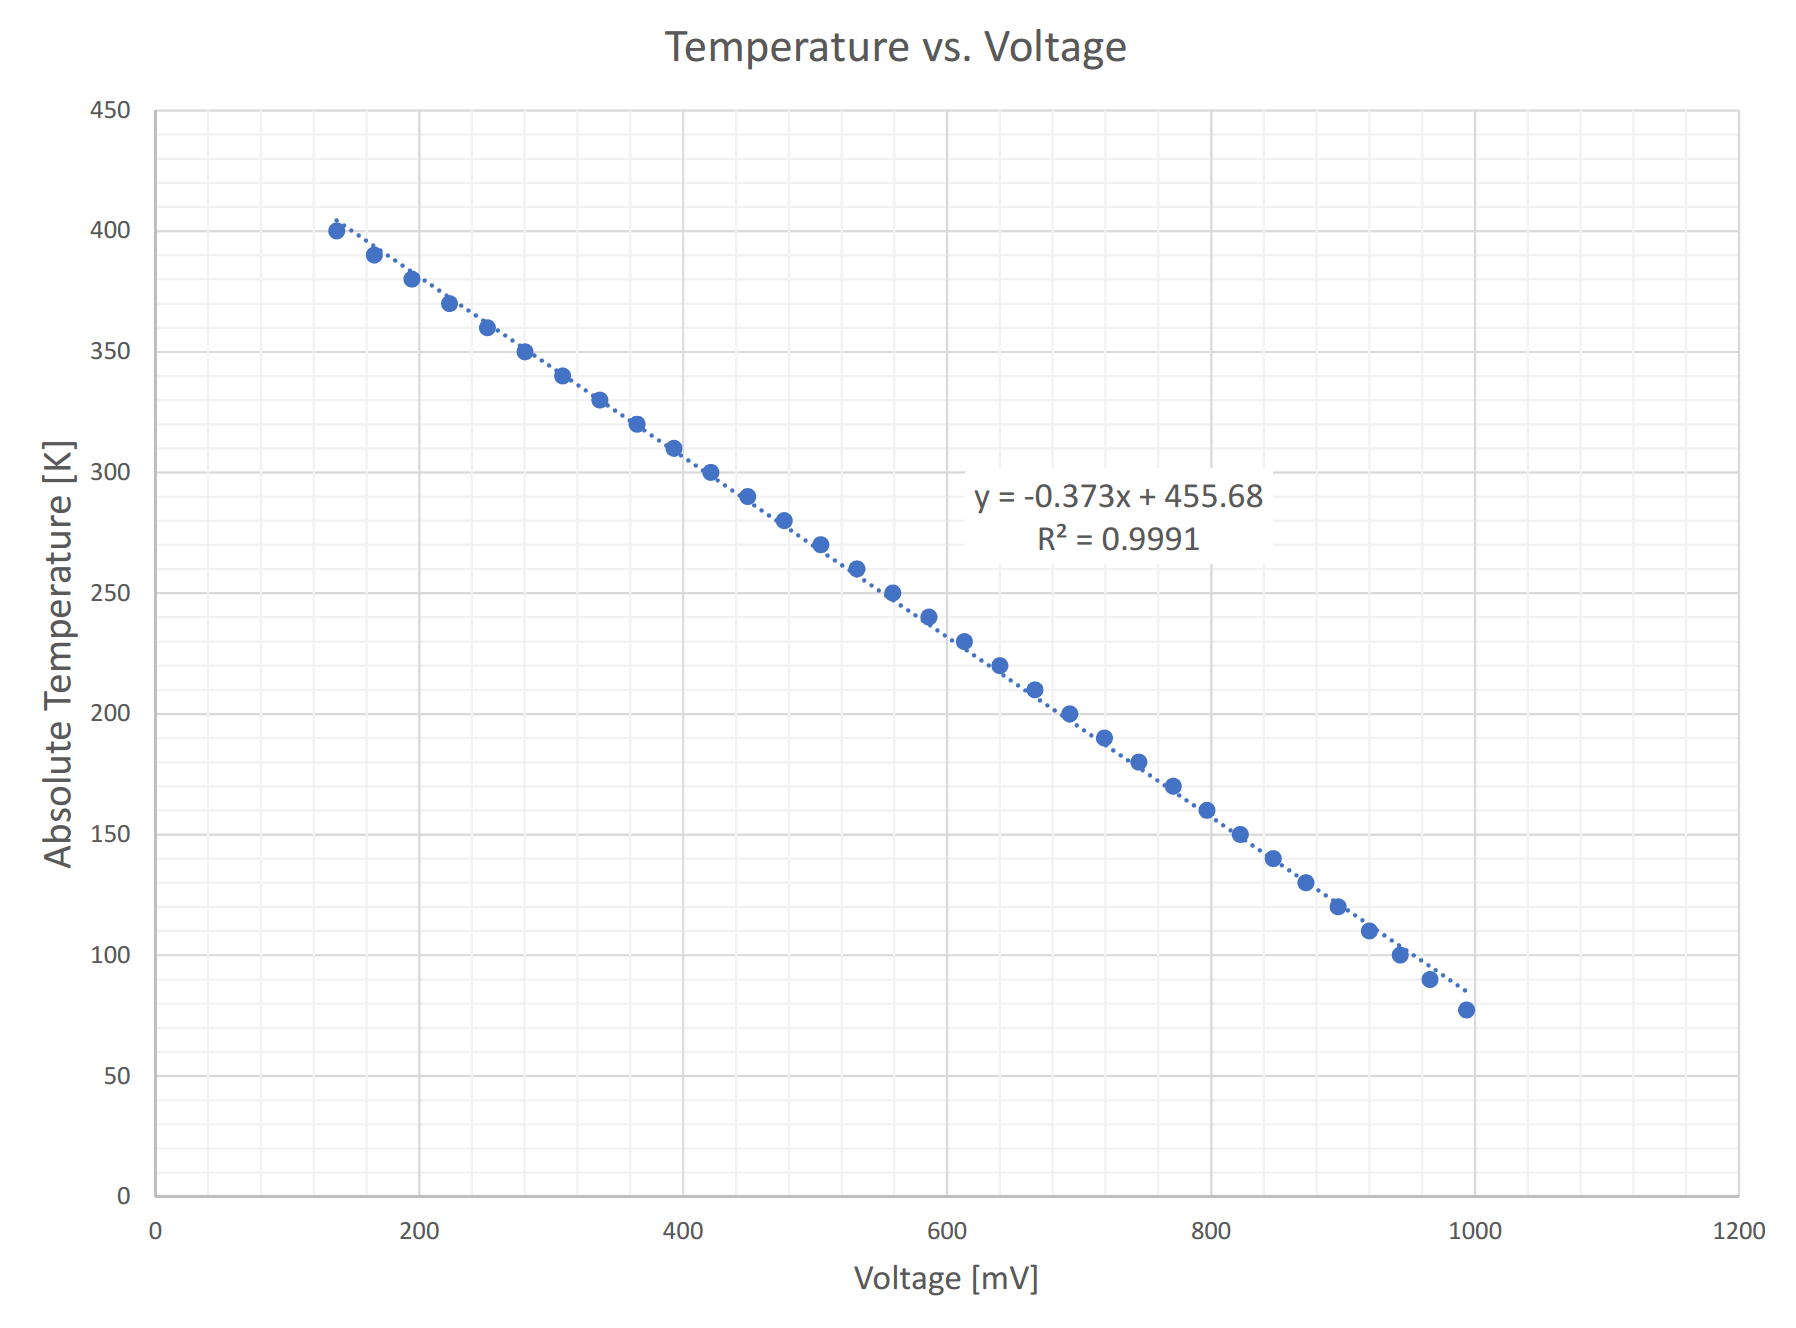
\includegraphics[width=0.7\textwidth]{TVConversion.PNG}
	\caption{Conversion between voltage and absolute temperature for a photodiode at constant $10 \ \mu A$ current.}
	\label{tvgraph}
\end{figure}


\begin{table}[H]
	\centering
	\begin{tabular}{c c c c} \toprule
		\textbf{Temp [K]} & $\mathbf{\delta}$\textbf{T [K]} & \textbf{Power [W]} & $\mathbf{\delta}$\textbf{S} \\ \toprule
		98.7 & 0.746 & 2.94E-18 & 1.29E-17 \\
		120  & 0.746 & 3.23E-18 & 1.28E-17 \\
		139  & 0.746 & 2.94E-18 & 2.58E-17 \\
		187  & 1.49  & 3.82E-18 & 1.27E-17 \\
		236  & 1.12  & 4.11E-18 & 2.53E-17 \\
		272  & 0.746 & 4.11E-18 & 2.53E-17 \\
		305  & 0.746 & 4.11E-18 & 1.27E-17 \\
		333  & 0.746 & 4.11E-18 & 1.27E-17 \\
		\bottomrule  
	\end{tabular}
	\caption{Temperature Dependence for R = 10 $\Omega$}
	\label{temp10}
\end{table}



\begin{table}[H]
	\centering
	\begin{tabular}{c c c c} \toprule
		\textbf{Temp [K]} & $\mathbf{\delta}$\textbf{T [K]} & \textbf{Power [W]} & $\mathbf{\delta}$\textbf{S} \\ \toprule
		98.3 & 0.746 & 5.52E-17 & 7.25E-18 \\
		115  & 0.746 & 6.78E-17 & 3.27E-17 \\
		141  & 0.746 & 8.22E-17 & 1.77E-17 \\
		190  & 1.49  & 1.14E-16 & 9.77E-18 \\
		230  & 1.12  & 1.38E-16 & 2.56E-17 \\
		280  & 0.746 & 1.56E-16 & 2.36E-17 \\
		304  & 0.746 & 1.74E-16 & 1.82E-17 \\
		337  & 0.746 & 1.90E-16 & 1.71E-17 \\
		\bottomrule
	\end{tabular}
\caption{Temperature Dependence for R = 10 k$\Omega$}
\label{temp10k}
\end{table}



\begin{table}[H]
	\centering
	\begin{tabular}{cccc} \toprule
		\textbf{Temp [K]} & $\mathbf{\delta}$\textbf{T [K]} & \textbf{Power [W]} & $\mathbf{\delta}$\textbf{S} \\ \toprule
		99.5 & 0.746 & 4.91E-16 & 1.63E-17 \\
		113  & 0.746 & 5.76E-16 & 1.35E-16 \\
		143  & 0.746 & 7.29E-16 & 5.49E-17 \\
		192  & 1.49  & 1.03E-15 & 4.86E-17 \\
		226  & 1.12  & 1.19E-15 & 1.82E-17 \\
		286  & 0.746 & 1.42E-15 & 2.72E-17 \\
		301  & 0.746 & 1.53E-15 & 1.63E-17 \\
		340  & 0.746 & 1.70E-15 & 2.98E-17 \\
		\bottomrule
	\end{tabular}
	\caption{Temperature Dependence for R = 100 k$\Omega$}
	\label{temp100k}
\end{table}


\subsection*{Shot Noise}

\begin{table}[H]
	\centering
	\begin{tabular}{cccc} \toprule
		$\mathbf{\Delta f}$ & $\mathbf{\delta (\Delta f)}$ & $\mathbf{\langle s \rangle}$ & $\mathbf{\delta \langle s \rangle}$ \\ \toprule
		314   & 12.56   & 9.68E-21 & 4.33E-22 \\
		984   & 39.36   & 1.97E-20 & 8.80E-22 \\
		3284  & 131.36  & 5.23E-20 & 2.34E-21 \\
		9984  & 399.36  & 1.42E-19 & 6.33E-21 \\
		32984 & 1319.36 & 4.60E-19 & 2.06E-20 \\
		99984 & 3999.36 & 1.38E-18 & 6.18E-20 \\
		\bottomrule
	\end{tabular}
	\caption{Data collected for power spectral density versus bandwidth for shot noise}
	\label{shotBandwidthTable}
\end{table}


\begin{table}[H]
	\centering
	\begin{tabular}{cccc} \toprule
		$\mathbf{I_{dc}}$ & $\mathbf{\delta (I_{dc})}$ & $\mathbf{\langle s \rangle}$ & $\mathbf{\delta \langle s \rangle}$ \\ \toprule
		1.00E-06 & 2.00E-07 & 3.21E-26 & 6.66E-27 \\
		2.00E-06 & 2.00E-07 & 9.62E-26 & 1.10E-26 \\
		3.00E-06 & 2.00E-07 & 1.16E-25 & 1.02E-26 \\
		4.00E-06 & 4.00E-07 & 1.48E-25 & 1.70E-26 \\
		5.00E-06 & 1.00E-07 & 1.76E-25 & 1.06E-26 \\
		6.00E-06 & 1.00E-07 & 2.00E-25 & 1.18E-26 \\
		7.00E-06 & 1.00E-07 & 2.44E-25 & 1.43E-26 \\
		8.00E-06 & 2.00E-07 & 2.80E-25 & 1.73E-26 \\
		9.00E-06 & 2.00E-07 & 3.17E-25 & 1.92E-26 \\
		1.00E-05 & 2.00E-07 & 3.65E-25 & 2.19E-26 \\
		\bottomrule
	\end{tabular}
	\caption{Data collected for power spectral density versus photodiode current for shot noise}
	\label{shotCurrentTable}
\end{table}